% Placeholder figures and tables for Editorial Manager builds.
% Replace stub graphics with final journal figures before submission.

\begin{figure}[p]
\centering
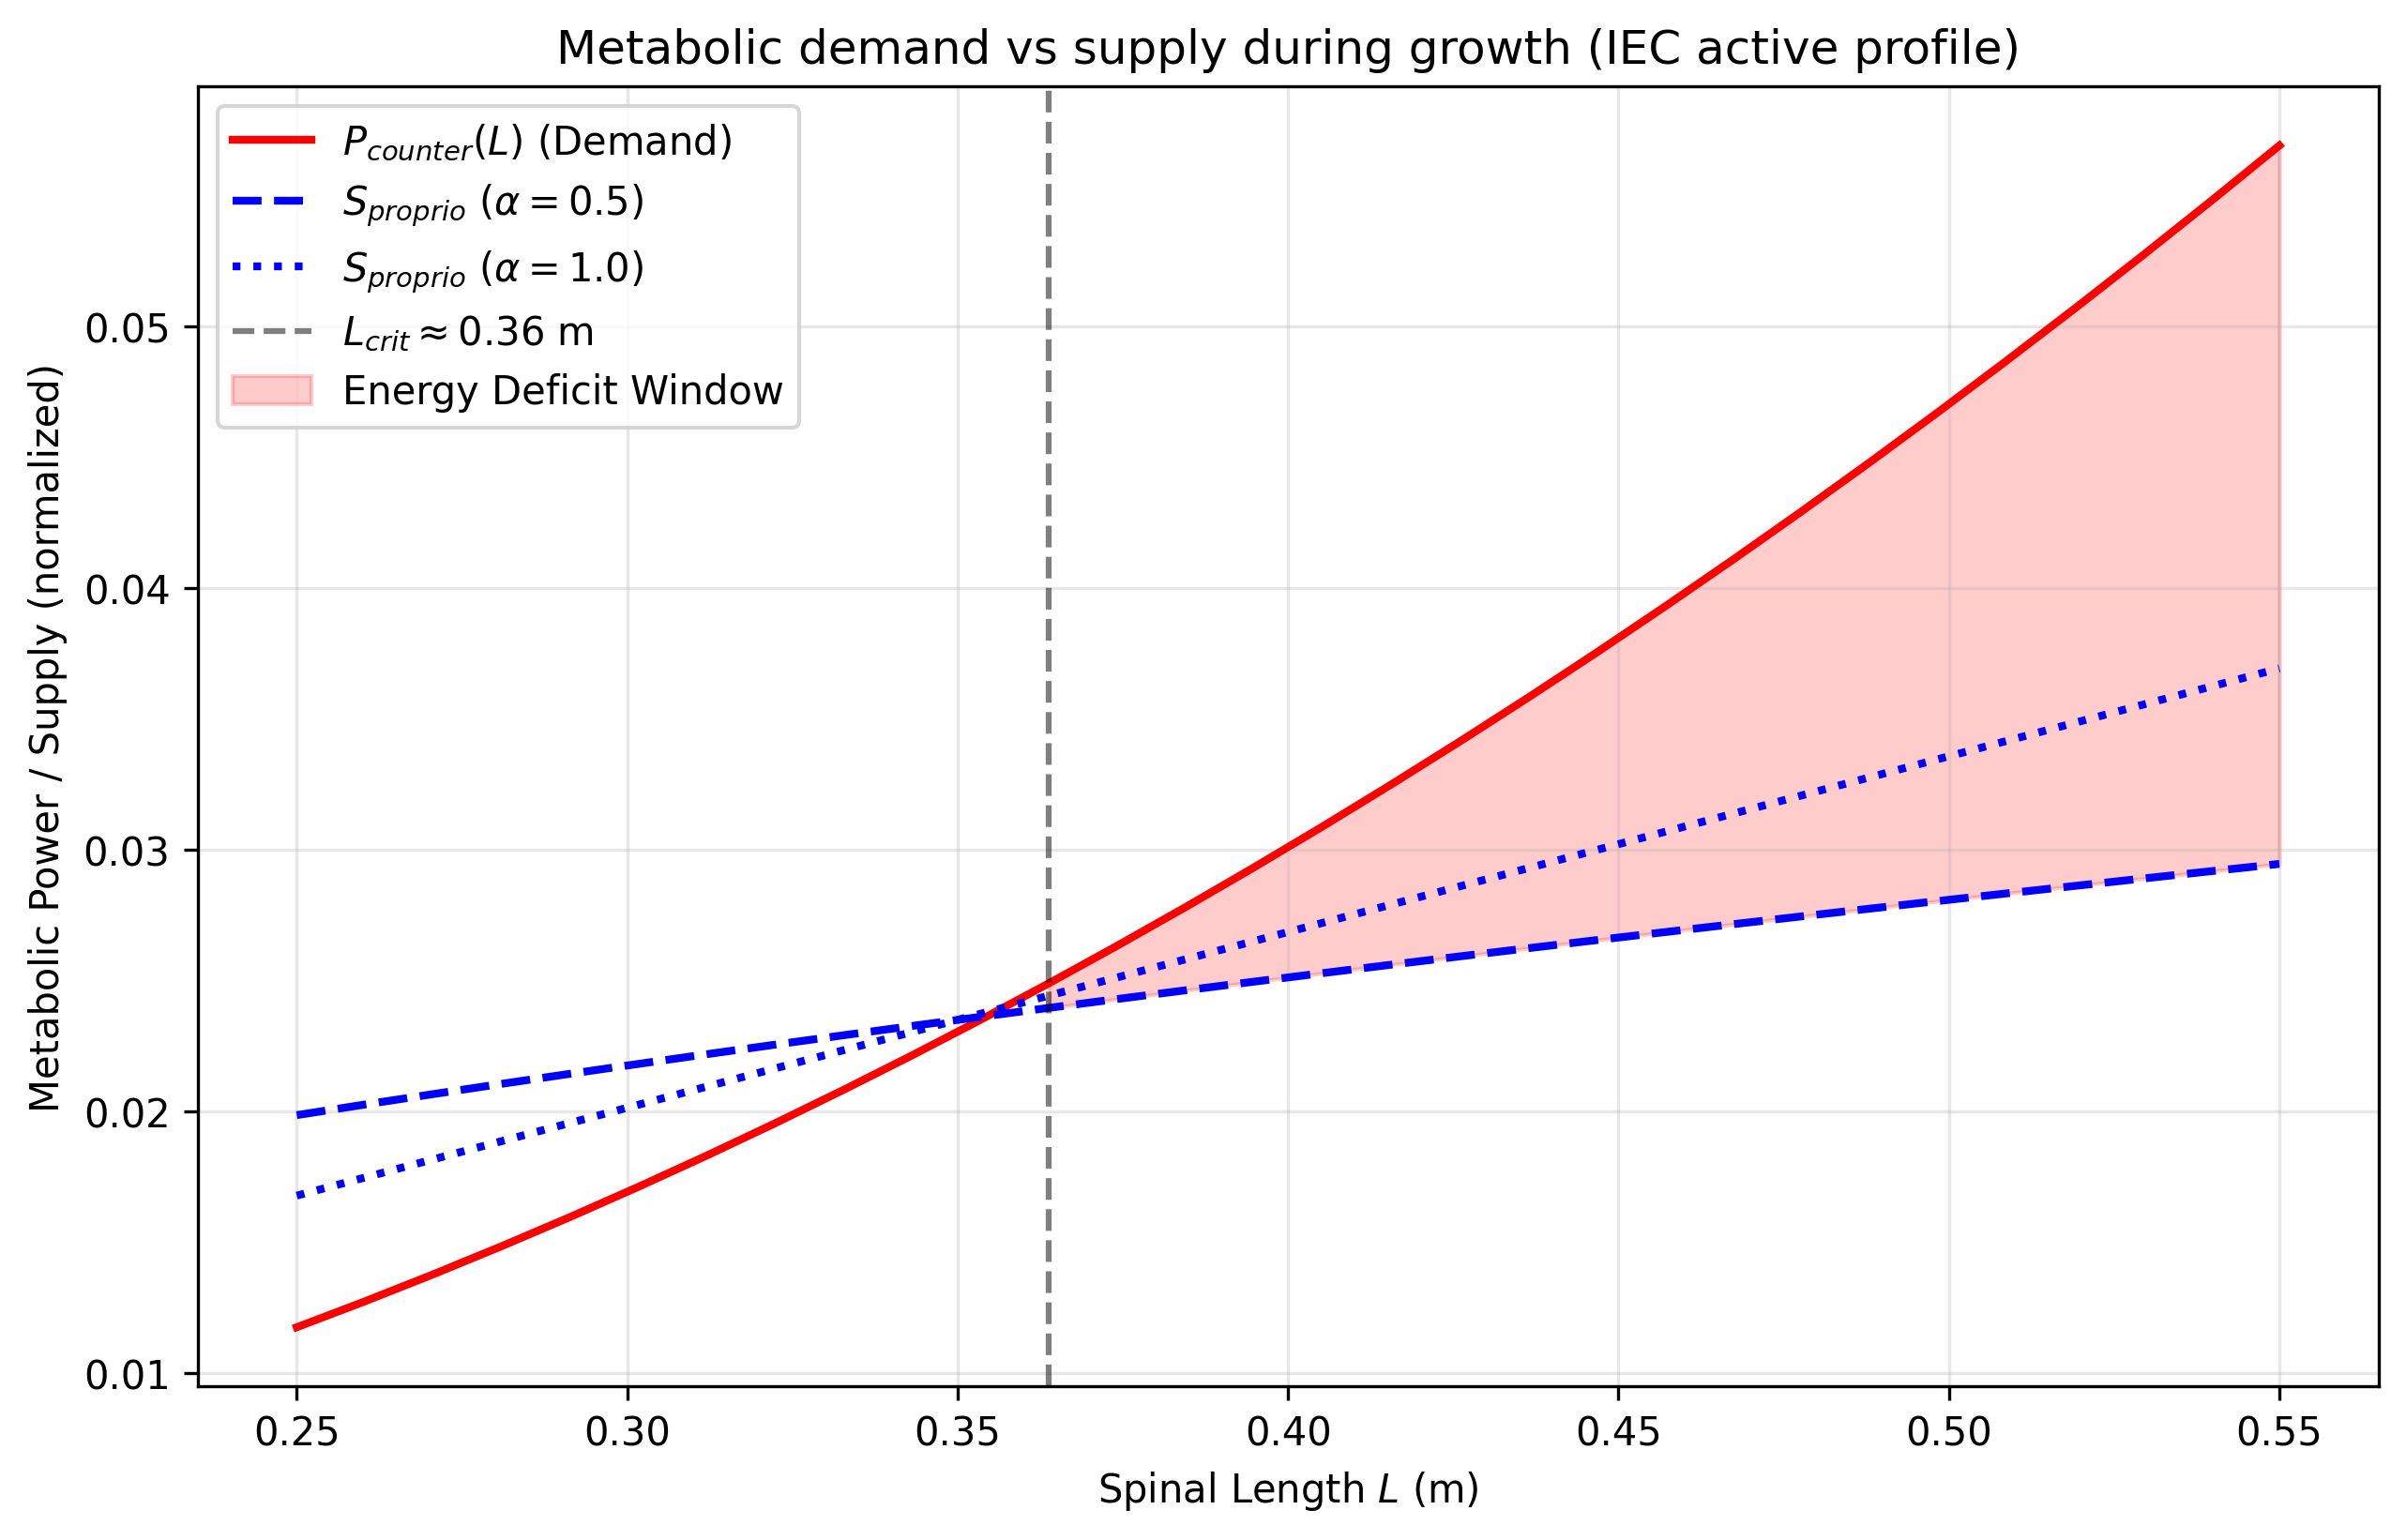
\includegraphics[width=0.85\textwidth]{../manuscript/figures/energy_deficit_window.png}
\caption{\textbf{Metabolic demand vs.\ supply during growth.} Placeholder using the repository energy-deficit window plot; replace with the final journal figure file if a vector version is required.}
\label{fig:energy_deficit_window}
\end{figure}

\begin{figure}[p]
\centering
\includegraphics[width=0.75\textwidth]{example-image-a}
\caption{\textbf{Placeholder:} mode spectrum / eigenmode analysis (replace with final Fig.).}
\label{fig:mode_spectrum}
\end{figure}

\begin{figure}[p]
\centering
\includegraphics[width=0.32\textwidth]{example-image-b}\hfill
\includegraphics[width=0.32\textwidth]{example-image-c}\hfill
\includegraphics[width=0.32\textwidth]{example-image-a}
\caption{\textbf{Placeholder:} IEC validation of sagittal S-curve in Cosserat simulations (replace with final multi-panel Fig.). Panels A--C are layout stubs; panel D referenced in text should be added in the final composite.}
\label{fig:iec_s_shape_validation}
\end{figure}

\begin{figure}[p]
\centering
\includegraphics[width=0.85\textwidth]{example-image-a}
\caption{\textbf{Placeholder:} scoliosis emergence / bifurcation diagram (replace with final Fig.).}
\label{fig:scoliosis_emergence}
\end{figure}

\begin{figure}[p]
\centering
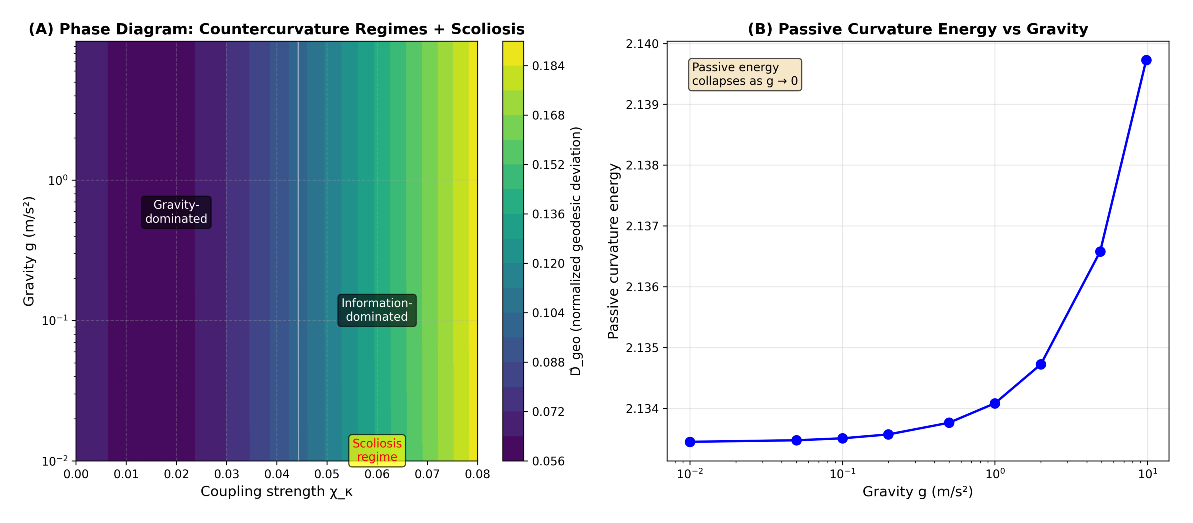
\includegraphics[width=0.85\textwidth]{../manuscript/fig_phase_diagram_scoliosis.pdf}
\caption{\textbf{Phase diagram} $(\chi_\kappa, g)$ from the repository generator (replace/caption for journal style if needed).}
\label{fig:phase_diagram}
\end{figure}

\begin{figure}[p]
\centering
\includegraphics[width=0.85\textwidth]{example-image-a}
\caption{\textbf{Placeholder:} protein morphology / demand--supply landscape (replace with final Fig.).}
\label{fig:morphology_landscape}
\end{figure}

\begin{figure}[p]
\centering
\includegraphics[width=0.85\textwidth]{example-image-a}
\caption{\textbf{Placeholder:} vector--scalar mismatch analysis (replace with final Fig.).}
\label{fig:vector_mismatch_analysis}
\end{figure}

\begin{table}[p]
\centering
\caption{Placeholder cross-species Bio-Gravitational Number summary (replace with final data table).}
\label{tab:cross_species}
\begin{tabular}{lcc}
\toprule
Species & Body mass (kg) & $\mathcal{B}_g$ (representative) \\
\midrule
Mouse & 0.02 & $>0.1$ \\
Human (adolescent) & 50 & $\approx 0.01$ \\
\bottomrule
\end{tabular}
\end{table}

\begin{table}[p]
\centering
\caption{Placeholder statistical summary referenced in the text (replace with final values).}
\label{tab:statistical_summary}
\begin{tabular}{lccc}
\toprule
Analysis & Metric & $p$-value & Note \\
\midrule
See main text & As reported & --- & Populate from final analysis \\
\bottomrule
\end{tabular}
\end{table}

\begin{table}[p]
\centering
\caption{Placeholder experiment sweep summary (replace with final simulation output table).}
\label{tab:experiment_results_summary}
\begin{tabular}{lcc}
\toprule
Condition & Cobb ($^\circ$) & Anisotropy ratio \\
\midrule
See main text & --- & --- \\
\bottomrule
\end{tabular}
\end{table}
